\section*{Membuat Aplikasi Websheet}
\begin{enumerate}
	
	\item Klik App Builder dan klik create 
	\begin{figure} [!htbp]
	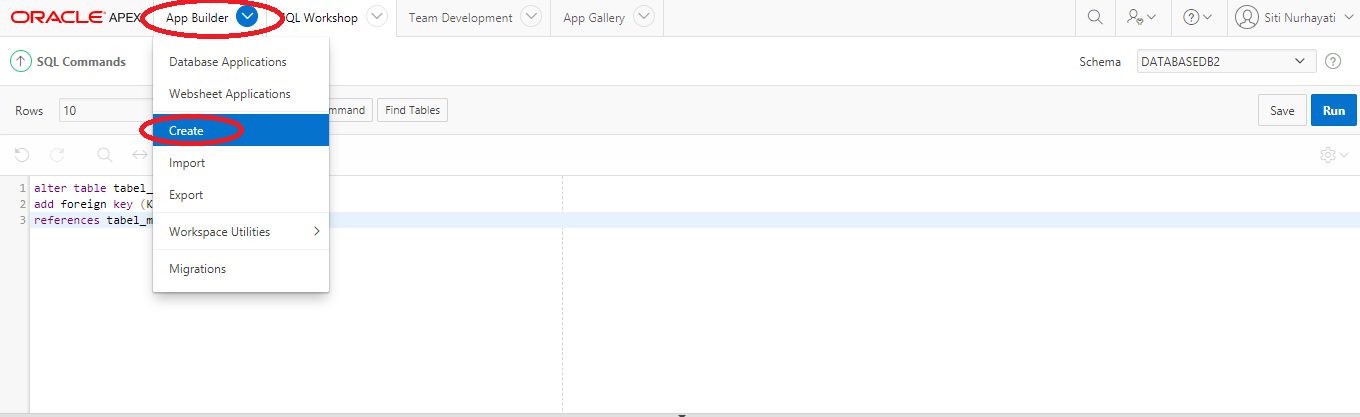
\includegraphics[scale=0.2]{Apex/21.png}
	\centering
	\end{figure}

	\item Klik New Aplication 
	\begin{figure} [!htbp]
	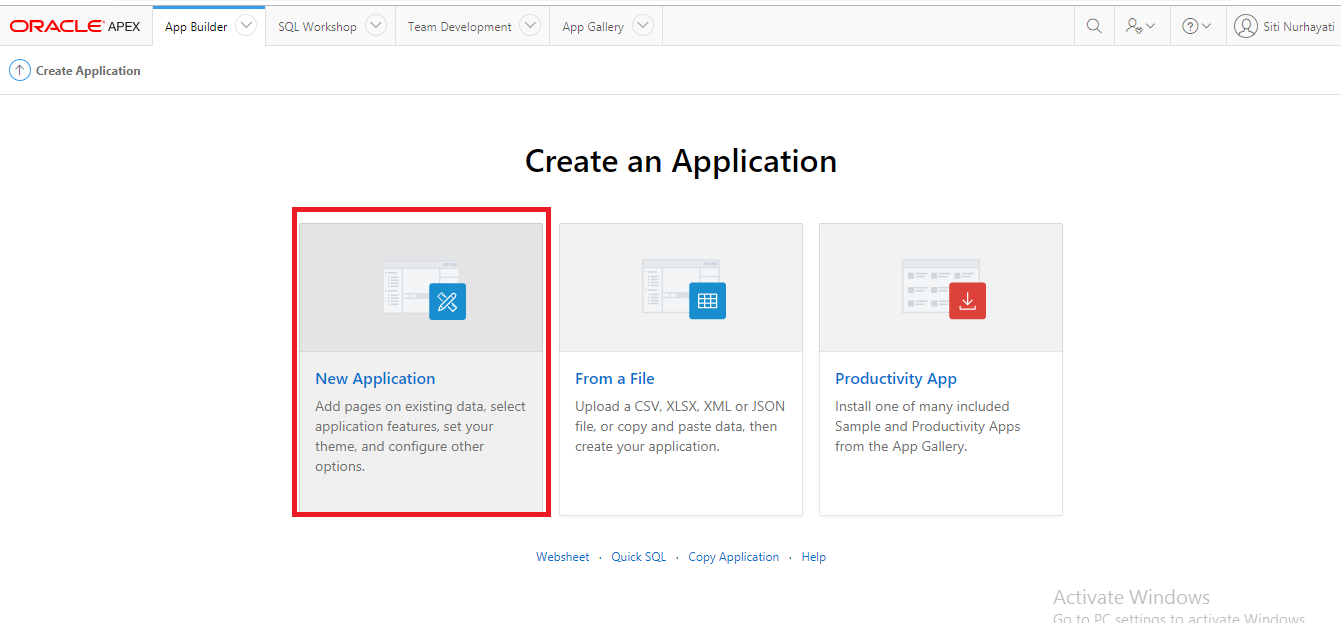
\includegraphics[scale=0.2]{Apex/22.png}
	\centering
	\end{figure}
	
	\item Tuliskan nama aplikasi yang anda inginkan 
	\begin{figure} [!htbp]
	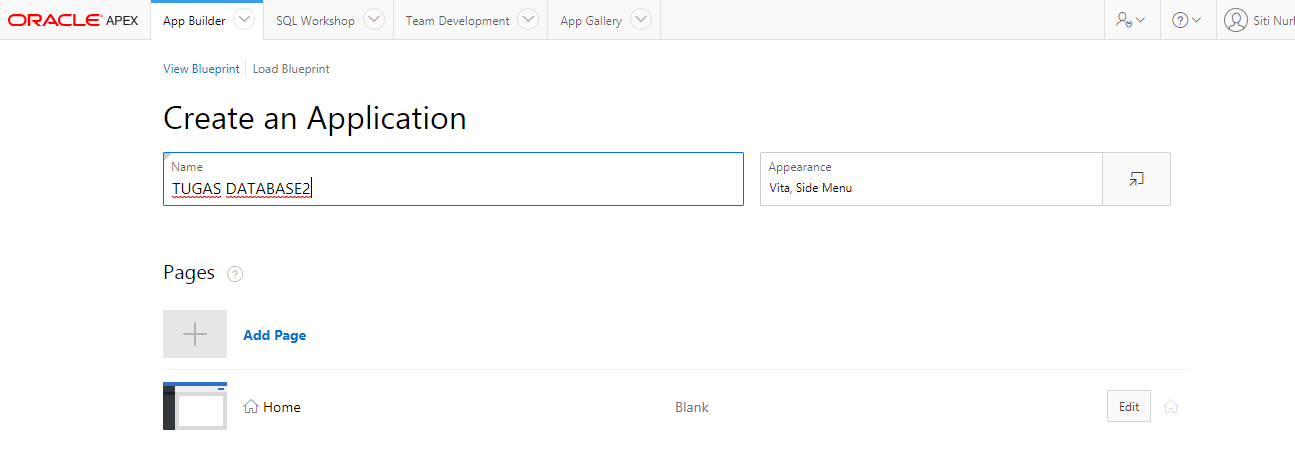
\includegraphics[scale=0.2]{Apex/23.png}
	\centering
	\end{figure}
	
	\item Untuk menambahkan page pada aplikasi klik "Add Page" lalu pilih "interactive report"
	\begin{figure} [!htbp]
	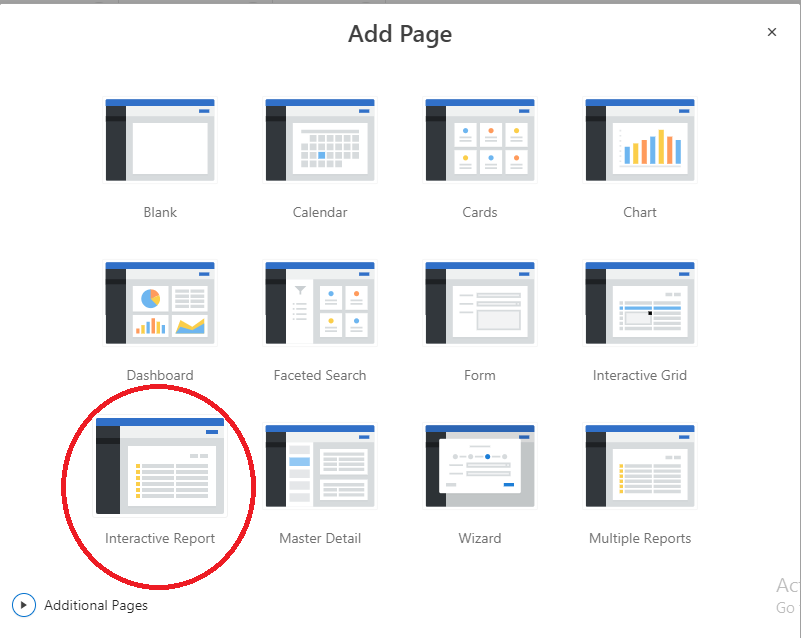
\includegraphics[scale=0.2]{Apex/24.png}
	\centering
	\end{figure}
	
	\item Isikan page name lalu di table or view klik tabel yang sesuai dengan page namanya lalu klik ad page. Lakukan pada tabel mhs, tabel dosen dan tabel matakuliah 
	\begin{figure} [!htbp]
	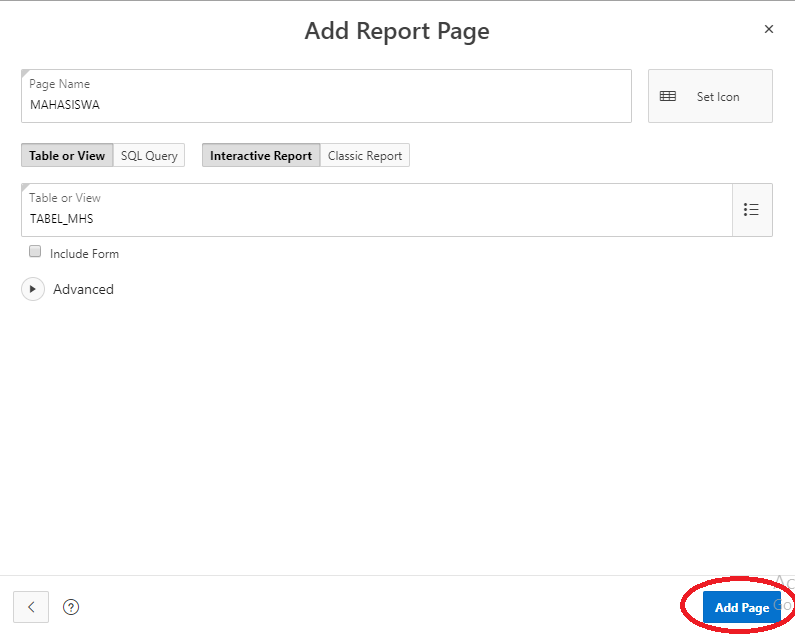
\includegraphics[scale=0.2]{Apex/25.png}
	\centering
	\end{figure}
	
	\item Pada Tabel Jadwal dan Tabel Nilai sedikit berbeda yaitu klik  SQL Query dan masukan Query seperti digambar 
	\begin{figure} [!htbp]
	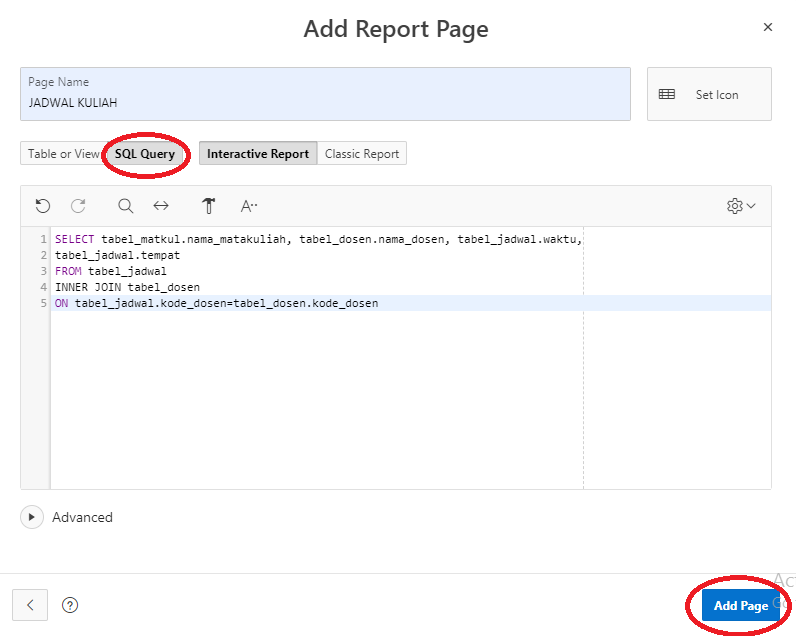
\includegraphics[scale=0.2]{Apex/27.png}
	\centering
	\end{figure}
	
	\begin{figure} [!htbp]
	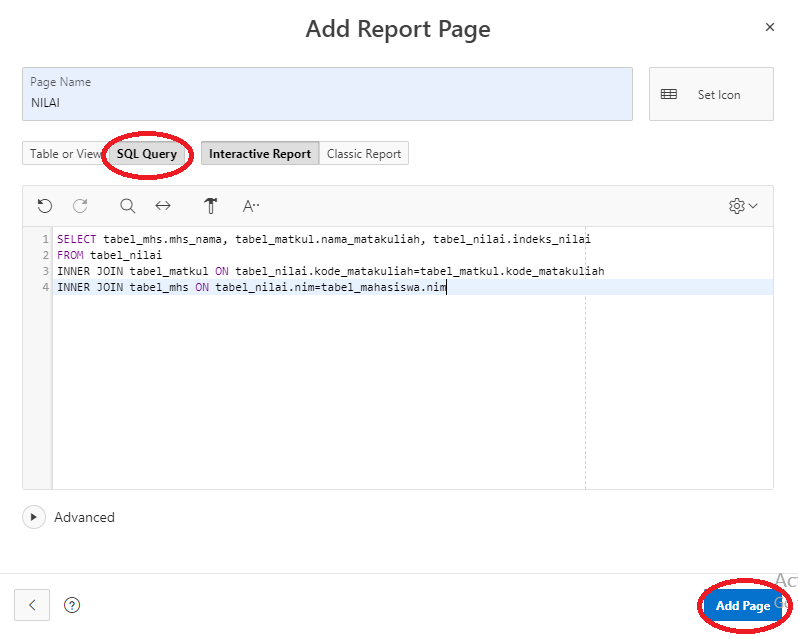
\includegraphics[scale=0.2]{Apex/28.png}
	\centering
	\end{figure}
	
	\item Lalu klik Create Application seperti digambar 
	\begin{figure} [!htbp]
	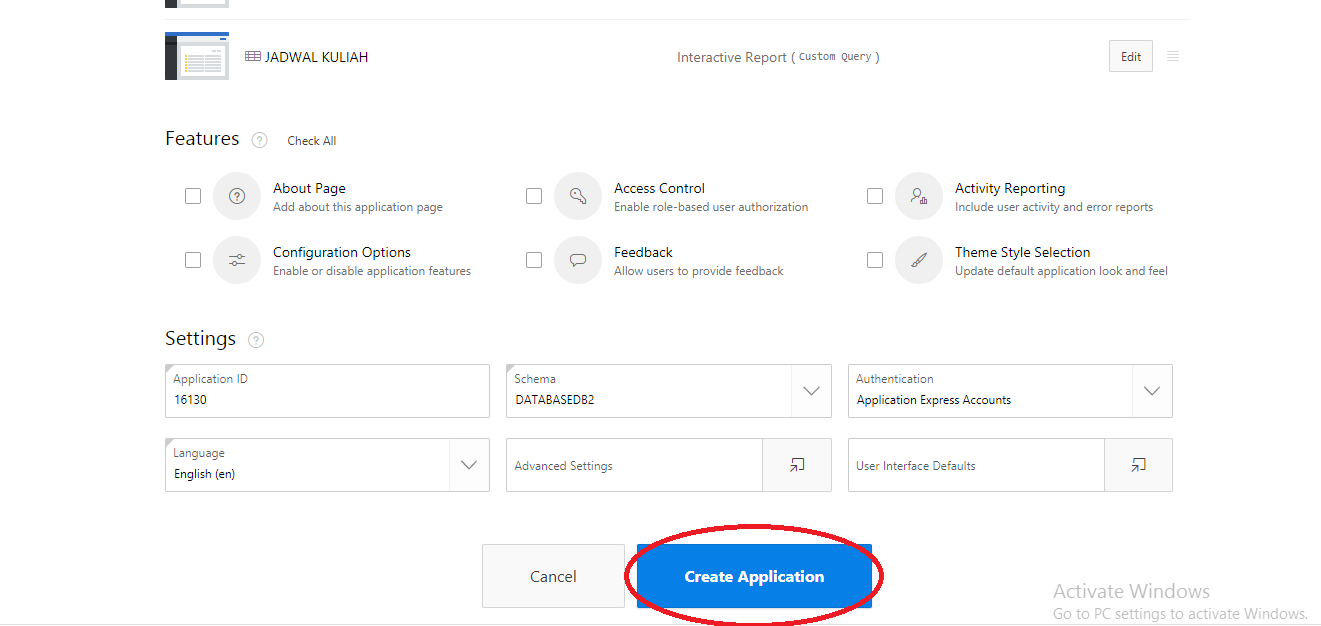
\includegraphics[scale=0.2]{Apex/29.png}
	\centering
	\end{figure}
	
	\item Lalu klik Run Application
	\begin{figure} [!htbp]
	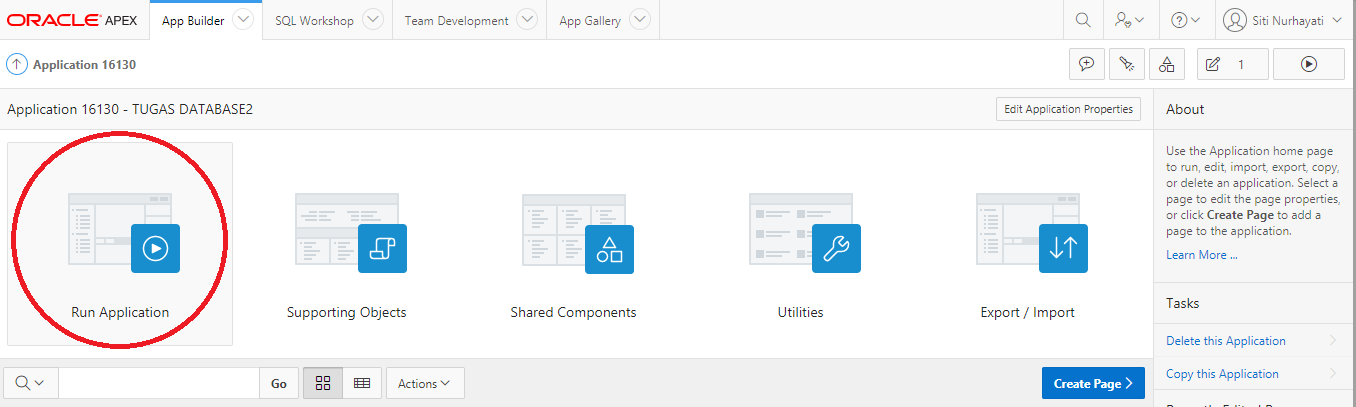
\includegraphics[scale=0.2]{Apex/30.png}
	\centering
	\end{figure}
	
	\item Masukan ulang username dan pasword untuk melanjutkan proses berikutnya  
	\begin{figure} [!htbp]
	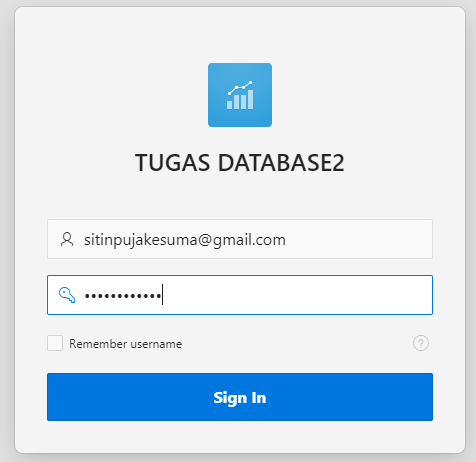
\includegraphics[scale=0.2]{Apex/31.png}
	\centering
	\end{figure}
	
	\item Aplikasi jadi   
	\begin{figure} [!htbp]
	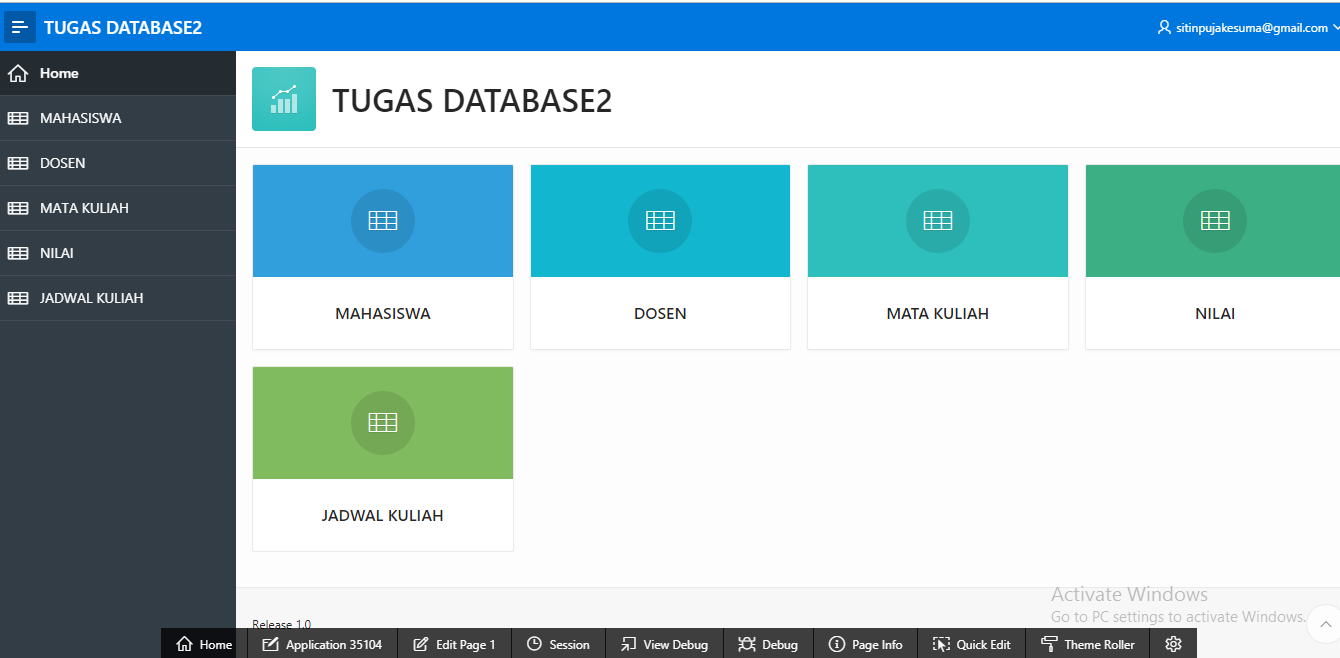
\includegraphics[scale=0.2]{Apex/32.png}
	\centering
	\end{figure}
	
Userid: sitinpujakesuma@gmail.com//
pasword: PUJAKESUMA11//
Workspace: databasedb2//
Link Aplication: https://apex.oracle.com/pls/apex/f?p=35104:6:700642050052135::NO:::
	
\end{enumerate}
